\documentclass[pressentation,9pt,aspectratio=1610,xcolor=table]{beamer}
\usepackage[utf8]{inputenc}
\usepackage[T1]{fontenc}
\usepackage{graphicx}
\usepackage{grffile}
\usepackage{longtable}
\usepackage{colortbl}
\usepackage{multicol}
\usepackage{wrapfig}
\usepackage{rotating}
\usepackage[normalem]{ulem}
\usepackage{amsmath}
\usepackage{textcomp}
\usepackage{amssymb}
\usepackage{capt-of}
\usepackage{hyperref}
\usepackage[english]{babel}
\usepackage{etex}
\usepackage{pifont}\usepackage{booktabs}
\usepackage{collcell}
\usepackage{tikz}
\usepackage{amsmath}
\usepackage{mathspec}
\usepackage{cancel}
\usepackage{pgfplots,pgfplotstable}
\usetikzlibrary{mindmap,trees,shapes,arrows,spy,3d,backgrounds,positioning,pgfplots.statistics,calc,fit,overlay-beamer-styles, decorations.markings,matrix}
\usepgfplotslibrary{groupplots}
\pgfplotsset{/pgf/number format/assume math mode=true}

% \defaultfontfeatures{Ligatures=TeX}\setmathsfont(Digits,Latin,Greek)[BoldFont=Fira Sans Bold]{Fira Sans Book}

\renewenvironment{description}{\begin{itemize}}{\end{itemize}}
\usepackage[type={CC}, modifier={by-sa}, version={4.0},]{doclicense}
\usetheme{metropolis}
\usecolortheme[snowy]{owl}
\metroset{progressbar=frametitle,numbering=fraction,titleformat=smallcaps,block=fill,sectionpage=simple,sectionpage=simple}
\setbeamercovered{again covered={\opaqueness<1->{25}}}

% Documents info
\title{Data Science for Geosciences}
\subtitle{Introduction}
\author{Florent Chatelain \inst{1} \and Mathieu Fauvel \inst{2}}
\institute{
  \inst{1} MCF Grenoble INP, GIPSA-lab \and %
  \inst{2} CR1 INRA, CESBIO
}
\date{14-18 January 2019\\Brest France}
\setbeamertemplate{footline}
{%
\leavevmode%
\hbox{\begin{beamercolorbox}[wd=.5\paperwidth,ht=2.5ex,dp=1.125ex,leftskip=.3cm plus1fill,rightskip=.3cm]{author in head/foot}%
\usebeamerfont{author in head/foot}\insertshortauthor: \insertshorttitle
\hfill%
\end{beamercolorbox}%
\begin{beamercolorbox}[wd=.5\paperwidth,ht=2.5ex,dp=1.125ex,leftskip=.3cm,rightskip=.3cm plus1fil]{title in head/foot}%
\usebeamerfont{title in head/foot}\hfill\insertframenumber/\inserttotalframenumber\hspace{2em}
\end{beamercolorbox}}%
\vskip0pt%
}
\setbeamercolor{lowcol}{fg=black,bg=gray!05}
\setbeamertemplate{blocks}[rounded][shadow=false,lower=lowcol]
\setbeamersize{text margin left  = 0.5cm}
\setbeamersize{text margin right = 0.5cm}
\setbeamertemplate{itemize item}[square]
\setbeamertemplate{itemize subitem}[triangle]
\setbeamertemplate{itemize subsubitem}{$\star$}
\setbeamertemplate{navigation symbols}{}

% les macros
\newcommand{\exampletext}[1]{{\textcolor{green}{#1}}}
\newcommand{\structuretext}[1]{{\textcolor{blue}{#1}}}

\newcommand{\bydef}{\stackrel{{def}}{=}}
\newcommand{\ici}{\tcb{$\blacktriangleright \;$}}
\newcommand{\icir}{\alert{$\blacktriangleright \;$}}
\newcommand{\iciex}{\exampletext{$\blacktriangleright \;$}}
\usepackage{pifont}
\newcommand{\doigt}{\noindent \Pisymbol{pzd}{43}}
\newcommand{\doigtr}{\alert{\noindent \Pisymbol{pzd}{43}}}
\newcommand{\doigtex}{{\exampletext{\noindent \Pisymbol{pzd}{43}}}}

\newcommand{\bx}{{\boldsymbol{x}}}
\newcommand{\bbeta}{{\boldsymbol{\beta}}}
\newcommand{\balpha}{{\boldsymbol{\alpha}}}
\newcommand{\bxi}{{\boldsymbol{\xi}}}



\DeclareMathOperator{\var}{var}
\DeclareMathOperator{\cov}{cov}
\DeclareMathOperator{\trace}{trace}
\DeclareMathOperator{\rank}{rank}
\DeclareMathOperator{\logit}{logit}
\DeclareMathOperator{\sign}{sign}


% Set graph path
\graphicspath{{./Figs/}}

\definecolor{c1}{rgb}{0,0,0.562}
\definecolor{c2}{rgb}{0,0,0.875}
\definecolor{c3}{rgb}{0,0.25,1}
\definecolor{c4}{rgb}{0,0.625,1}
\definecolor{c5}{rgb}{0,1,1}
\definecolor{c6}{rgb}{0.375,1,0.625}
\definecolor{c7}{rgb}{0.688,1,0.312}
\definecolor{c8}{rgb}{1,0.938,0}
\definecolor{c9}{rgb}{1,0.562,0}
\definecolor{c10}{rgb}{1,0.188,0}
\definecolor{c11}{rgb}{0.812,0,0}
\definecolor{c12}{rgb}{0.5,0,0}


\begin{document}
\maketitle
\pgfplotsset{compat=newest}


\begin{frame}
  \frametitle{The presenters}
  \begin{block}{Florent Chatelain}
    \begin{itemize}
    \item Ph.D. degree in signal processing from the National Polytechnic Institute, Toulouse, France, in 2007
    \item Post-doc position at INRIA - ARIANA Team, 2007-2008
    \item Since 2008, Associate Professor at GIPSA-Lab, University of Grenoble, France.
    \item Research interests are centered around estimation, detection and large scale inference
    \end{itemize}
  \end{block}

  \begin{block}{Mathieu Fauvel}
    \begin{itemize}
    \item Ph.D. degree in signal and image processing from the National Polytechnic Institute, Grenoble, France, and the University of Iceland, in 2007
    \item Post-doc position at INRIA - MISTIS Team, 2008-2010
    \item Assistant Professor (Grenoble, 2007-2008 \& Toulouse, 2010-2011)
    \item Associate Professor at DYNAFOR, National Polytechnic Institute, Toulouse, between 2011-2018.
    \item Since 2018, Research (CR1) at CESBIO, INRA.
    \item Research interests are: machine learning for environmental/ecological monitoring
    \end{itemize}
  \end{block}
\end{frame}

\section{What is machine learning?}


\begin{frame}[fragile]{Machine Learning $\subset$ Artificial Intelligence}
  \begin{center}
    \begin{tikzpicture}
      \draw[fill=yellow!40] (2.75,0) ellipse (6.4 and 3.2);
      \draw[fill=blue!40] (1,0) ellipse (4 and 2);
      \draw[fill=red!30] (-1,0) ellipse (1.6 and 0.8);

      \draw (5,2) node {\textbf{Artificial Intelligence}};
      \draw (2,1) node {\textbf{Machine Learning}};
      \draw (-0.75,0) node {\textbf{Deep Learning}};
    \end{tikzpicture}
  \end{center}
  {\tiny Taken from \url{https://www.geospatialworld.net/blogs/difference-between-ai%EF%BB%BF-machine-learning-and-deep-learning/}}
\end{frame}

\begin{frame}{Objective}
  \begin{center}
    \emph{How to extract knowledge or insights from data ?}
  \end{center}
  Learning problems are at the cross-section of several applied fields and science disciplines
  \begin{itemize}
  \item \emph{Machine learning} arose as a subfield of
    \begin{itemize}
    \item Artificial Intelligence,
    \item Computer Science.
    \end{itemize}
    Emphasis on large scale implementations and applications: \textcolor{blue}{algorithm centered}
  \item  \emph{Statistical learning} arose as a subfield of
    \begin{itemize}
    \item Statistics,
    \item Applied Maths,
    \item Signal Processing, \ldots
    \end{itemize}
    Emphasizes models and their interpretability: \textcolor{blue}{model centered}
  \end{itemize}
\end{frame}


\begin{frame}
  \frametitle{Definitions of Learning}
  
  \begin{block}{Machine Learning in Computer Science}
    
    Tom Mitchell (The Discipline of Machine Learning, 2006)
    \medskip
    
    A computer program CP is said to learn from \structuretext{experience E} with respect to
    some class of \structuretext{tasks T} and \structuretext{performance measure P}, if its performance at
    tasks in T, as measured by P, improves with experience E 
  \end{block}
    
    
  \begin{block}{Key points}
    \begin{itemize}
    \item<2-> Experience E:  \structuretext{data and statistics}
    \item<3-> Performance measure P: \structuretext{optimization}
    \item<4-> tasks T: utility 
      \begin{itemize}
      \item automatic translation
      \item playing Go
      \item ... doing what human does
      \end{itemize}
    \end{itemize}
    
  \end{block}    
\end{frame}

\begin{frame}
  \frametitle{Experience E: the data!}
  
  \begin{block}{Type of data:  qualitatives / ordinales / quantitatives variables}
    \begin{description}
    \item Text:  strings
    \item Speech: time series
    \item Images/videos: 2/3d dependences 
    \item Networks: graphs
    \item Games: interaction sequences
    \item ...
    \end{description}
  \end{block}
  
  \begin{block}{Big data (volume, velocity, variety, veracity)}
    Data are available without having decided to collect them!
    \begin{itemize}
    \item importance of preprocessings (cleaning up, normalization, coding,...)
    \item importance of a good representation : from raw data to vectors
    \end{itemize}
  \end{block}
\end{frame}


\begin{frame}
  \frametitle{Objective and performance measures P}
  
  \begin{block}{Generalize}
    \begin{itemize}
    \item Perform well (minimize P) on \alert{new data} (fresh data, i.e. unseen during learning)
    \item[\doigt]  Derive good (P/error rate) prediction functions
    \end{itemize}    
  \end{block}

  \visible<2>{
    \begin{tabular}{cc}
      
\includegraphics[width=0.4\textwidth]{blue-fish}& 
\includegraphics[width=0.4\textwidth]{blue-elephant}\\
      A fish & A fish
    \end{tabular}
  }
  
\end{frame}


\begin{frame}{References}
  \begin{block}{Reference books}
    \begin{thebibliography}{9}
      \setbeamertemplate{bibliography item}[book]
    \bibitem{A} Trevor Hastie, Robert Tibshirani et Jerome Friedman (2009), \normalcolor{The Elements of Statistical Learning (2nd Edition)}, \color{gray}{\it Springer Series in Statistics}
    \bibitem{B} Christopher M. Bishop (2007), \normalcolor{Pattern Recognition and Machine Learning}, \color{gray}{\it Springer}
    \bibitem{C} Kevin P. Murphy (2012), \normalcolor{Machine Learning: a Probabilistic Perspective}, \color{gray}{\it MIT press}
    \end{thebibliography}
  \end{block}
  
  \begin{block}{\normalcolor{Supplementary materials, datasets, online courses, ...}}
    \begin{thebibliography}{9}
      \setbeamertemplate{bibliography item}[online]
    \bibitem{A} \url{http://www-stat.stanford.edu/~tibs/ElemStatLearn/}
    \bibitem{B} {\small \url{https://www.cs.ubc.ca/~murphyk/MLbook/} }
    \bibitem{D} \url{https://www.coursera.org/course/ml} \color{gray}{\scriptsize \it very popular MOOC (Andrew Ng)}
    \bibitem{E} \url{https://work.caltech.edu/telecourse.html} \color{gray}{\scriptsize \it more involved MOOC (Y. Abu-Mostafa)}
      \bibitem{F} \url{https://scikit-learn.org/stable/auto_examples/index.html} \color{gray}{\scriptsize \it Examples from the sklearn library}
    \end{thebibliography}
  \end{block}
\end{frame}



\section{Examples}
\begin{frame}
  \frametitle{Recognition of handwritten digits (US postal envelopes)}
    \begin{center}
      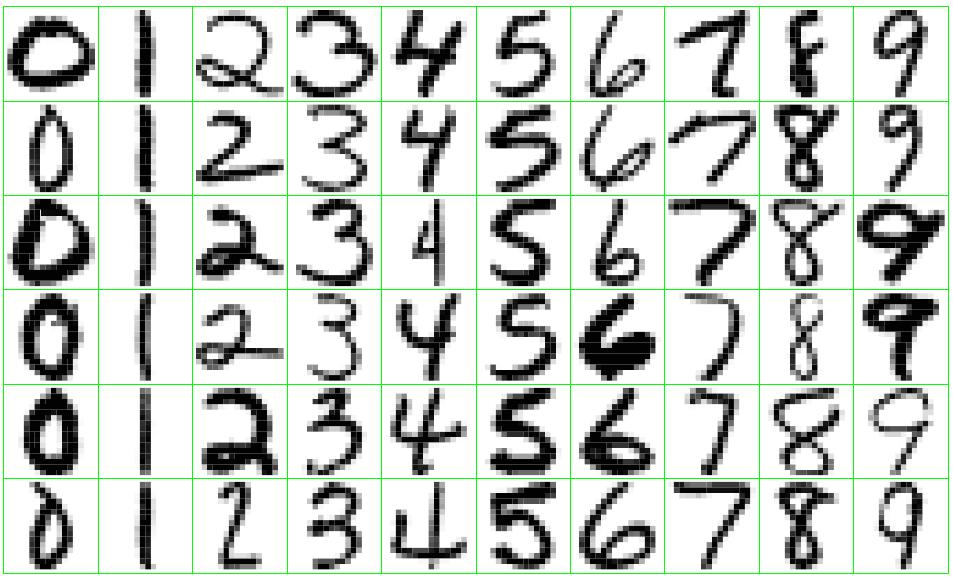
\includegraphics[width=.5\textwidth]{ex_handwriten.jpg}
    \end{center}
    \begin{itemize}
    \item[\doigt] Predict the class (0,...,9) of each sample from an image of 
      $16\times 16$ pixels, with a pixel intensity coded from $0$ to $255$
    \item Low error rate to avoid wrong allocations of mails!
    \end{itemize}
    \begin{center}
      \alert{Supervised classification }
    \end{center}
\end{frame}

\begin{frame}
  \frametitle{Spams Recognition}
    \begin{center}
      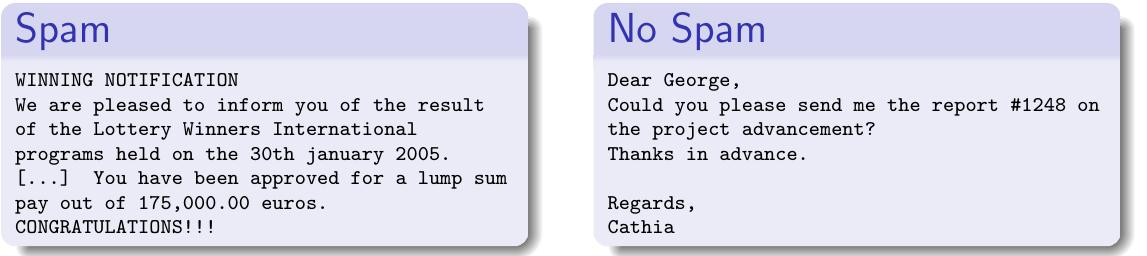
\includegraphics[width=.8\textwidth]{ex_spams.jpg}
    \end{center}
    \begin{itemize}
    \item[\doigt] 
      Define a model to predict whether an email is spam or not
    \item Low error rate to avoid deleting useful messages, or filling the mailbox with useless emails
    \end{itemize}
  \begin{center}
    \alert{supervised classification}
  \end{center}
  
\end{frame}


\begin{frame}{Recognition of Hekla Volcano landscape, Iceland}

  \begin{columns}
    \begin{column}{0.45\columnwidth}
      \begin{center}
        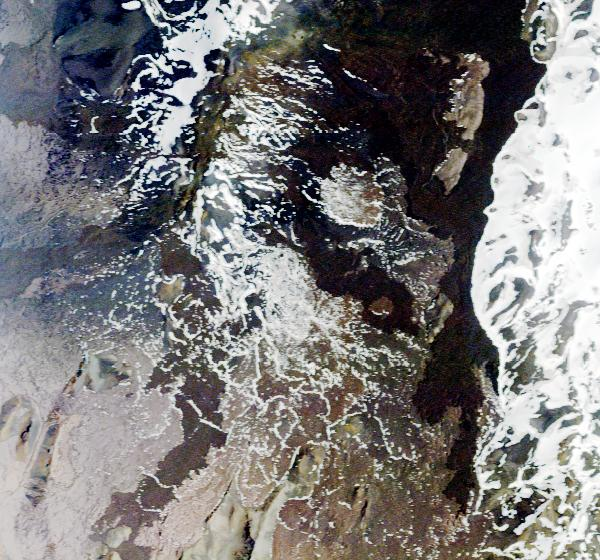
\includegraphics[width=.8\linewidth]{hekla_original.jpg}
      \end{center}
    \end{column}
    \begin{column}{0.45\columnwidth}
      \begin{center}
        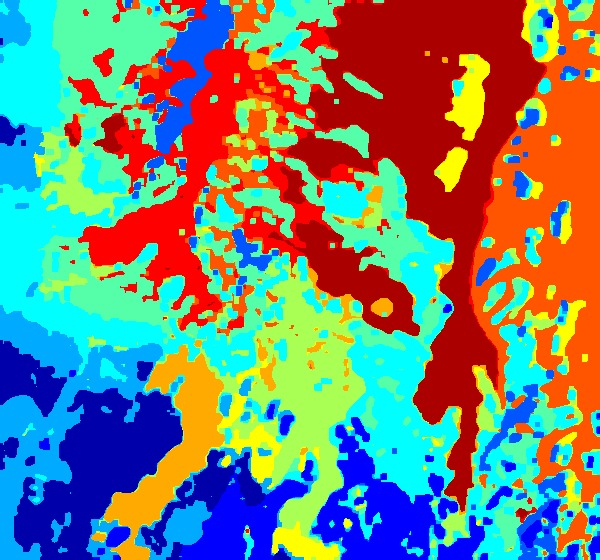
\includegraphics[width=.8\linewidth]{hekla_classif.jpg}
      \end{center}
    \end{column}
  \end{columns}
  
  \begin{itemize}
  \item[\doigt] Predict the class of landscape $\in \{$ \textcolor{c1}{Lava 1970}, \textcolor{c2}{Lava 1980 I}, \textcolor{c3}{Lava 1980 II},  \textcolor{c4}{Lava 1991 I}, \textcolor{c5}{Lava 1991 II}, \textcolor{c6}{Lava moss cover}, \textcolor{c7}{hyaloclastite formation}, \textcolor{c8}{Tephra lava}, \textcolor{c9}{Rhyolite}, \textcolor{c10}{Scoria}, \textcolor{c11}{Firn-glacier ice}, \textcolor{c12}{Snow} $\}$ from digital remote sensing images
    % \item Low error rate to avoid deleting useful messages, or filling the mailbox with useless emails
  \end{itemize}

\begin{center}
  \alert{supervised or unsupervised classification}
\end{center}
\end{frame}


\begin{frame}{Prediction of El Niño southern oscillation}
  \begin{center}
    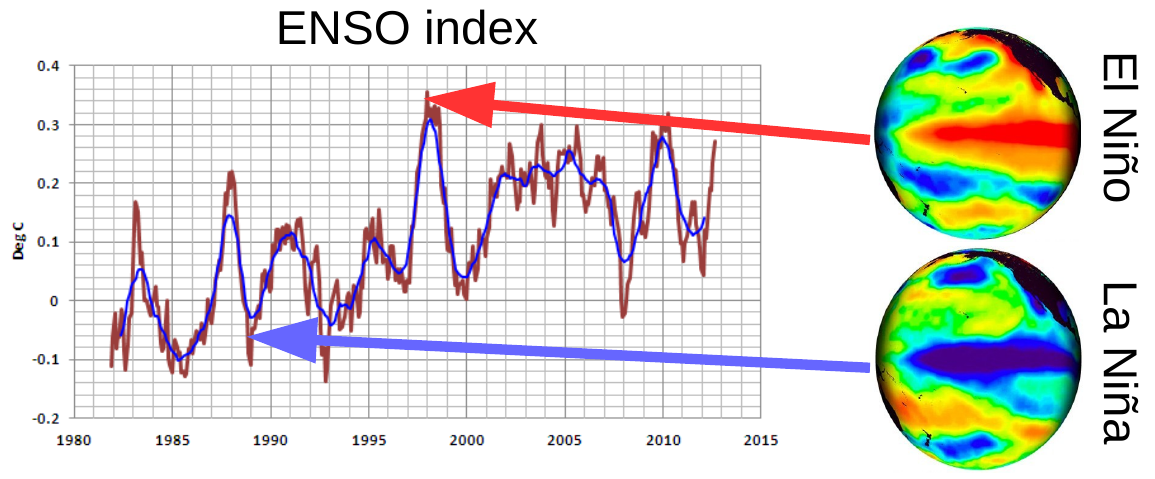
\includegraphics[width=.8\linewidth]{ENSO_Nino_Nina.png}
  \end{center}
  
  \begin{itemize}
  \item[\doigt] Predict, 6 months in advance, the intensity of an El Niño Southern Oscillation (ENSO) event from ocean-atmosphere datasets (sea level pressure, surface wind components, sea surface temperature, surface air temperature, cloudiness...)
  \end{itemize}
  \begin{center}
    \alert{supervised regression}
  \end{center}
\end{frame}


\begin{frame}{Recognition of fish sounds}

  \begin{center}
    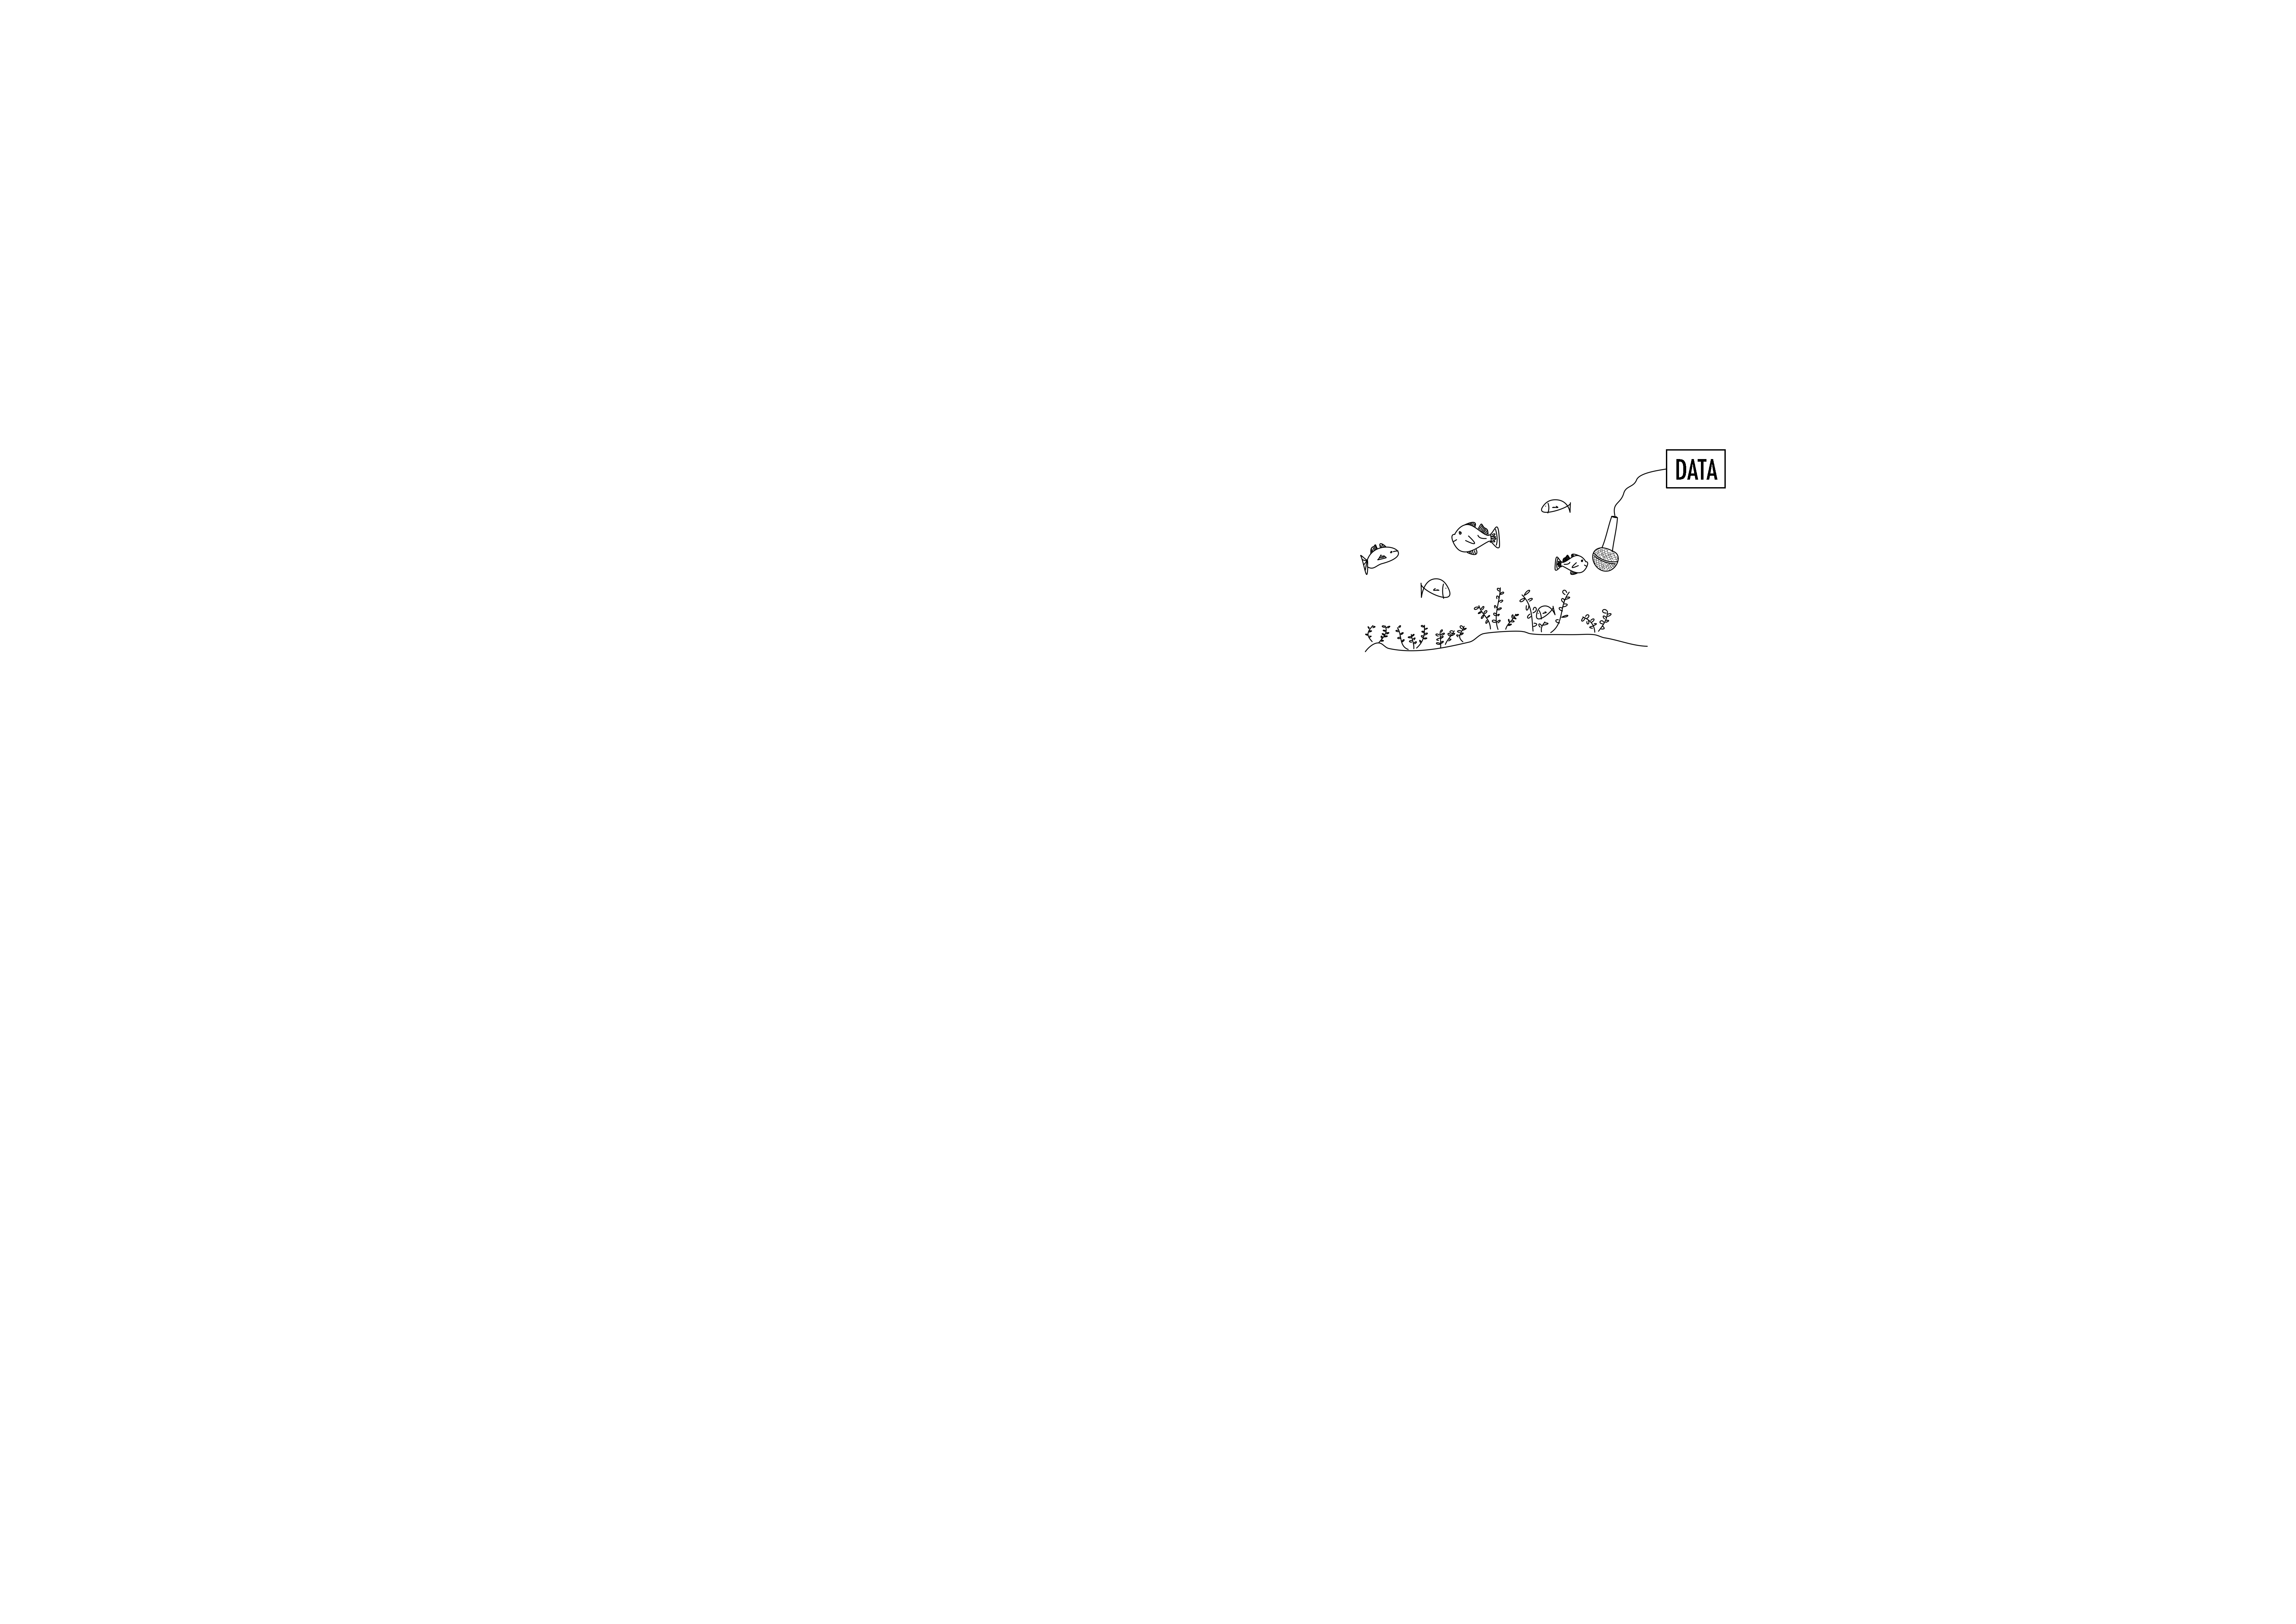
\includegraphics[keepaspectratio=true,width=.3\textwidth]{get_data.pdf}
    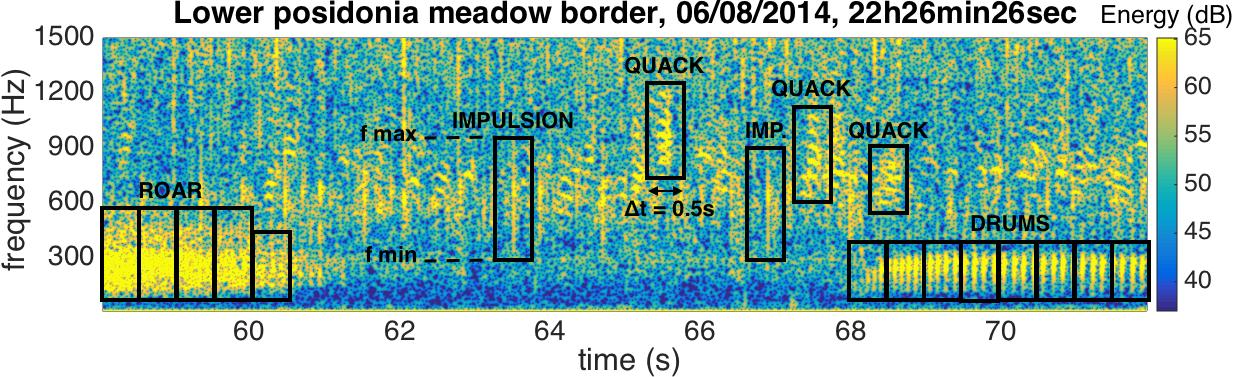
\includegraphics[keepaspectratio=true,width=0.7\textwidth]{spectro_global_top_16384-small.jpg}
  \end{center}
  \begin{itemize}
  \item[\doigt] Predict the class of underwater sounds (roar, quack, drums, impulsion) from  times series recorded by hydrophones ($f_s=156kHz$)
  \end{itemize}

  \begin{center}
    \alert{supervised or unsupervised classification}
  \end{center}
  
\end{frame}

\begin{frame}{Prediction of galaxy spectrum}

  \begin{center}
    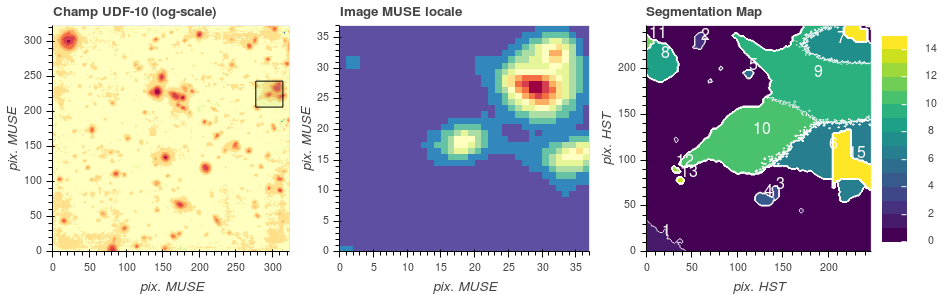
\includegraphics[width=.8\textwidth]{screenshot-whiteimages.png} \\
  \end{center}
  \begin{itemize}
  \item[\doigt] Predict galaxy spectra from both hyperspectral MUSE datacubes and Hubble Space Telescope images for better understanding of the early universe
  \end{itemize}
  \begin{center}
    \alert{supervised regression}
  \end{center}
\end{frame}

\begin{frame}{Recognition of climate-ocean events}

  \begin{center}
    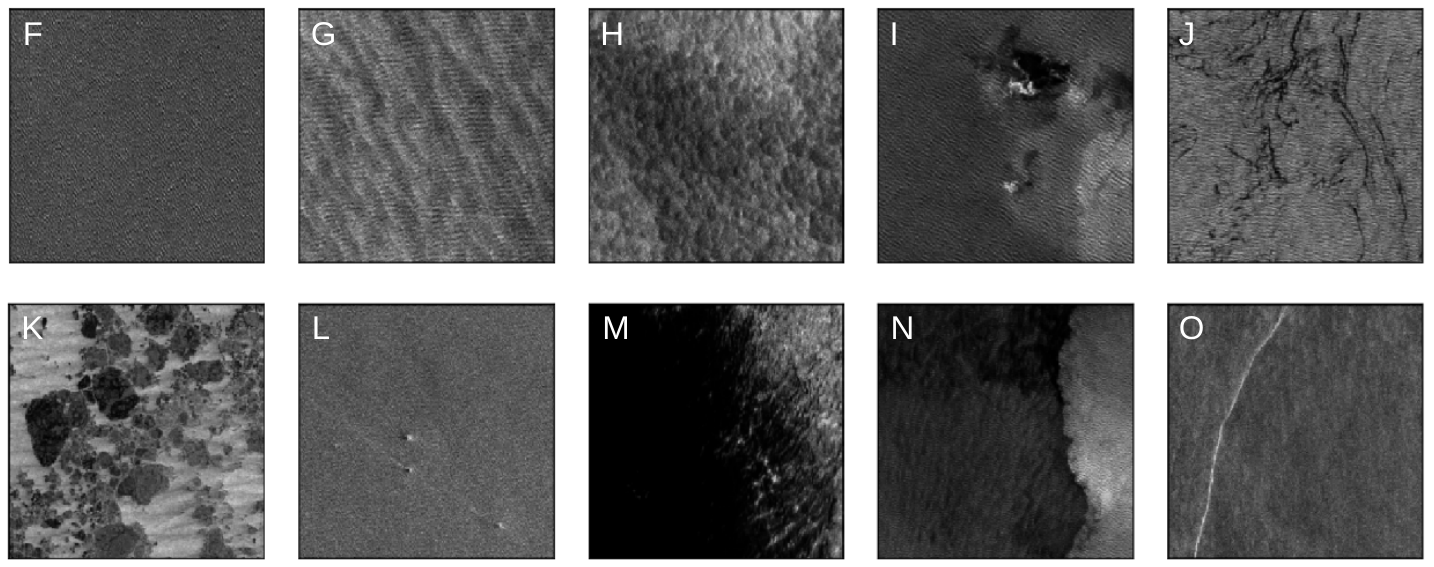
\includegraphics[keepaspectratio=true,width=0.7\textwidth]{SAR_classes.png}
  \end{center}
  \begin{itemize}
  \item[\doigt] Predict the classes of SAR images  of the ocean (convective cells in I, sea ice in K, weather front in N,...) to detect
    climate-ocean events from water surface roughness 
  \end{itemize}
  
  \begin{center}
    \alert{supervised or unsupervised classification}
  \end{center}
  
\end{frame}


\section{Basics}
\begin{frame}
  \frametitle{Definitions}
  \begin{block}{Variable terminology}
    \begin{itemize}
    \item Observed data referred to as {\em input} variables, {\em predictors} or {\em features}: \textcolor{blue}{$X$}
    \item Data to predict referred to as {\em output} variables, or {\em responses}: \textcolor{blue}{$Y$}
    \end{itemize}
  \end{block}
  
  \begin{block}{Type of prediction problem: regression vs classification}
    Depending on the type of the {\em output} variables
    \begin{itemize}
    \item When $Y$ are \structuretext{quantitative} data (e.g. ENSO intensity index values): \structuretext{regression}
    \item When $Y$ are \structuretext{categorical} data (e.g. handwritten digits $Y\in \{0,\ldots,9\}$): \structuretext{classification}
    \end{itemize}\medskip
    
    Two very close problems
  \end{block}
\end{frame}

\begin{frame}
  \frametitle{Prediction problem}
  \begin{block}{Assumptions}
    \begin{itemize}
    \item Input variables $X_i$ are vectors in $\mathbb{R}^p$:
      \begin{align*}
        X_i= \left(X_{i,1}, \ldots, X_{i,p} \right)^T \in \mathcal{X} \subset \mathbb{R}^p
      \end{align*}
    \item Output variables $Y_i$ take values:
      \begin{itemize}
      \item In $\mathcal{Y \subset \mathbb{R}}$ (regression)
      \item In a finite set $\mathcal{Y}$ (classification)
      \end{itemize}
    \item \(Y = f(X) + \epsilon\)
    \end{itemize}
  \end{block}
  \begin{block}{Prediction rule}
    Function of prediction / rule of classification $\equiv$ function $\hat{f}: \  \mathcal{X} \rightarrow \mathcal{Y}$  to  
    get  predictions of new elements $Y$ given $X$
     $$\structuretext{\widehat{Y}=\hat{f}(X)}$$
  \end{block}
\end{frame}

\begin{frame}
  \frametitle{Supervised or unsupervised learning}

  \structuretext{Training set} $\equiv$ available sample  $\mathcal{T}$ to learn the prediction rule $f$ \medskip 
  
  For a sized $n$ training set, different cases:
  \begin{itemize}
  \item \structuretext{Supervised learning}:  $ \mathcal{T} \equiv \left\{ (X_1,Y_1), \ldots, (X_n,Y_n) \right\}$ are available
  \item \structuretext{Unsupervised learning}: $ \mathcal{T} \equiv \left( X_1, \ldots, X_n \right)$ are available only 
  \item \structuretext{Semi-supervised}: mixed scenario (often encountered in practice, but less information than in the supervised case)
  \end{itemize} 
\end{frame}

\section{Toy Example}

\begin{frame}{Binary classification}
  \begin{center}
    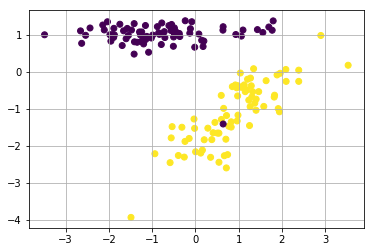
\includegraphics[width=0.5\textwidth]{academic_linear.png}
  \end{center}
\end{frame}
  
\begin{frame}
  \frametitle{Simple linear model for classification}
  We seek a prediction model based on the linear regression of the outputs 
  $Y \in \{-1,1\}$~:
  \begin{align*}
    Y & = \beta_1 X_1 + \beta_2 X_2 + \epsilon,
  \end{align*}
  where $\boldsymbol{\beta}=(\beta_1, \beta_2)^T $ is a 2D unknown parameter vector 
  
  \begin{block}{Learning problem $\Leftrightarrow$ Estimation of $\boldsymbol{\beta}$}
    {\it Least Squares Estimator} $\hat{\boldsymbol{\beta}}=(\hat{\beta}_1, \hat{\beta}_2)^T $: 
    minimize the training error rate (quadratic cost sense)
    $$
    RSS ( \boldsymbol{\beta} )= \sum_{i=1}^N (Y_i - \beta_1 X_{i,1} - \beta_2 X_{i,2} )^2
    $$
  \end{block}
  
  
  \begin{block}{Classification rule based on least squares regression}
    \vspace{-2mm}
    \begin{align*}
      f(X) &= \begin{cases}
        1 \textrm{ if } \structuretext{\widehat{Y}= \hat{\beta}_1 X_1 + \hat{\beta}_2 X_2} \ge 0,\\
        -1 \textrm{ otherwise}
      \end{cases}
    \end{align*}
  \end{block}

  \alert{Notebook}
\end{frame}
  
\begin{frame}
  \frametitle{Model complexity}
  Most of methods have a complexity related to their {\it effective} number of parameters

  \begin{block}{Linear classification: model order $p$}
  E.g. $d$th degree polynomial regression: $p=d+1$ parameters $a_k$ s.t.
    \begin{align*}
       Y &= \beta_0 + \beta_1 x + \beta_2 x^{2} + \ldots + \beta_d x^{d} + \epsilon,\\
       &= \boldsymbol{X}_d \boldsymbol{\beta}_d + \epsilon,
    \end{align*}
    where
    \begin{align*}
       \boldsymbol{X}_d &= \left[1, \;  x, \;  x^2, \ldots, x^d\right], \\
       \boldsymbol{\beta}_d &= \left[\beta_0, \beta_1, \beta_2, \ldots, \beta_d\right]^T.
    \end{align*}

  \end{block}
  \alert{Notebook}
\end{frame}

\begin{frame}
  \frametitle{Test error vs Train Error}
  
  \begin{minipage}{.45\textwidth}
    \begin{center}
      Error rate vs polynomial order $d$\\
      \alert{Notebook} 
    \end{center}
  \end{minipage}
  \begin{minipage}{.54\textwidth}
    \begin{itemize}
    \item Training error rate (i.e. error rate for train data used for learning) minimized when $d=19$
    \item True error rate (i.e. error rate for test data not used for learning) minimized when $d=5$ ...
  \end{itemize}
\end{minipage}

\begin{itemize}
\item[\doigt] Training error always decrease with the model complexity. \alert{Can't use alone to select the model!}
\end{itemize}


\end{frame}

\begin{frame}
  \frametitle{Model Selection}
  \begin{block}{Fundamental trade-off}
    \begin{itemize}
    \item Too simple model (high bias) $\rightarrow$ \alert{under-fitting}
    \item Too complex model (high variance) $\rightarrow$ \alert{over-fitting}
    \end{itemize}
  \end{block}
  \begin{center}
    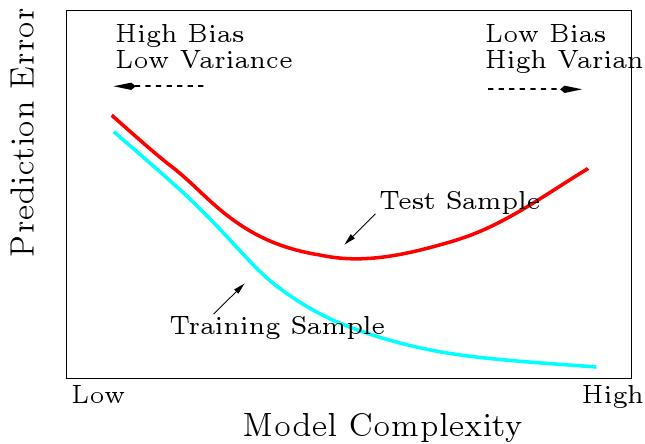
\includegraphics[width=.6\textwidth]{compromis.jpg}
  \end{center}
\end{frame}


\begin{frame}
  \frametitle{Fundamental Bias-Variance trade-off}
  %\begin{block}{Bias-Variance trade-off}
  If the true model is 
  $$ Y= f(X) + \epsilon,$$
  then for any prediction rule $\widehat{f}(X)$, 
  Mean Squared Error (MSE) expresses as
  $$
  E\left[ \left(Y- \widehat{f}(x) \right)^2 \right] = 
  \textrm{Var}\, \left[ \widehat{f}(x) \right] +  \textrm{Bias}\, \left[ \widehat{f}(x) \right]^2 + \textrm{Var}\, \left[ \epsilon \right] 
  $$
  \begin{itemize}
   \item $ \textrm{Var}\, \left[ \epsilon \right] $ is the {\em irreducible} part
  \end{itemize}
  \begin{itemize}
     \item as the flexibility of $\widehat{f}$ $\nearrow$, its variance $\nearrow$ and the bias $\searrow$
     \item[\doigtr] \alert{overfitting/underfitting trade-off}
  \end{itemize}
  %\end{block}
\end{frame}

\begin{frame}[label=conclusion,standout,noframenumbering]{}
\begin{center}
Thank you for your attention
\end{center}
\end{frame}
\begin{frame}[]{}
\begin{center}
\small
\doclicenseLongText

\doclicenseImage
\end{center}
\end{frame}
\end{document}

%%% Local Variables:
%%% mode: latex
%%% TeX-master: "main"
%%% End:
%%% latexmk -xelatex -shell-escape presentation_fauvel.tex